\subsection{Decoding Intermodulation Distortion: What’s Your Method?}

\begin{tcolorbox}[colback=gray!10, colframe=black, title=E4B10]

Which of the following methods measures intermodulation distortion in an SSB transmitter?
\begin{enumerate}[label=\Alph*.]
    \item Modulate the transmitter using two RF signals having non-harmonically related frequencies and observe the RF output with a spectrum analyzer.
    \item \textbf{Modulate the transmitter using two AF signals having non-harmonically related frequencies and observe the RF output with a spectrum analyzer.}
    \item Modulate the transmitter using two AF signals having harmonically related frequencies and observe the RF output with a peak reading wattmeter.
    \item Modulate the transmitter using two RF signals having harmonically related frequencies and observe the RF output with a logic analyzer.
\end{enumerate} \end{tcolorbox}

\subsubsection{Related Concepts}

Intermodulation distortion (IMD) occurs when two or more signals are mixed together in a nonlinear system, such as an SSB transmitter. The nonlinearity causes the creation of additional frequency components that are combinations (sums and differences) of the input frequencies. These additional frequencies can interfere with the original signals and create distortion.

To accurately measure IMD, it is important to use signals that are not harmonically related, as harmonic frequencies can lead to confusion in identifying distortion products. In this case, audio frequency (AF) signals are used, as they provide a simpler method for measuring and analyzing the distortion that occurs in the transmitter's output.

\subsubsection{Calculation Steps}

While the question does not explicitly require a calculation, understanding the principles behind how IMD is assessed involves the following steps:

1. \textbf{Set Up the Transmitter}: Use two audio signals \( f_1 \) and \( f_2 \) that are non-harmonically related.
2. \textbf{Modulate the SSB Transmitter}: Apply these signals to the transmitter to generate the modulated output. 
3. \textbf{Analyze with Spectrum Analyzer}: Connect a spectrum analyzer to the output of the transmitter. 
4. \textbf{Identify IMD Products}: Observe the output spectrum and record additional frequency components that appear in the transmission output that are not present in the input signals. These additional components are the intermodulation products.

\subsubsection{Diagram}

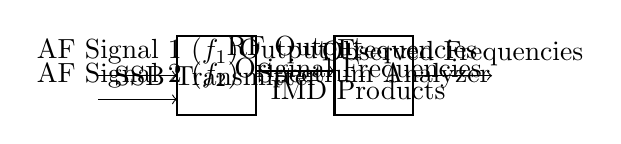
\begin{tikzpicture}
    % Draw transmitter
    \draw[thick] (0,0) rectangle (1,1) node[midway] {SSB Transmitter};
    
    % Draw input signals
    \draw[->] (-1,0.5) -- (0,0.5) node[midway, above] {AF Signal 1 ($ f_1 $)};
    \draw[->] (-1,0.2) -- (0,0.2) node[midway, above] {AF Signal 2 ($ f_2 $)};
    
    % Draw output signals
    \draw[->] (1,0.56) -- (2,0.56) node[midway, above] {RF Output};
    
    % Example frequencies in RF Output
    \node at (2.3,0.8) {Output Frequencies};
    \node at (2.3,0.56) {Original Frequencies};
    \node at (2.3,0.32) {IMD Products};
    
    % Draw spectrum analyzer
    \draw[thick] (2,0) rectangle (3,1) node[midway] {Spectrum Analyzer};
    \draw[->] (3,0.5) -- (4,0.5) node[midway, above] {Observed Frequencies};
\end{tikzpicture}
